\documentclass[a4paper]{article}
\usepackage[utf8x]{inputenc}
\usepackage[margin=1.7in]{geometry}
\RequirePackage[utf8]{inputenc}
\usepackage{graphicx}


\begin{document}
\title{Compilateur Deca: Documentation de l'extension: Optimisation}
\author{\'Equipe 58}
\maketitle
\section{Introduction}
Pour notre compilateur Decac nous avons dû choisir une extension parmi plusieurs extensions possibles, et notre choix s'est porté sur l'optimisation. L'optimisation consiste à rendre un code plus performant, de donner de meilleurs résultats, ou y arriver plus vite ou avec le moins de ressources possibles, c'est à dire à l'exécuter plus rapidement en faisant moins d'opérations au niveau du processeur, ou des opérations qui sont plus rapides.Plusieurs types d'optimisation de code sont possibles et ont été déjà implémentées, il s'agissait donc pour nous de reprendre ces méthodes classiques et en utiliser dans notre propre compilateur.
\section{Spécification de l'extension Optimisation}
\subsection{Optimisations implémentées}
Voici la liste des différentes spécifications de l'optimisation:
\begin{itemize}
\item \texttt{DeadStore} \\
      \texttt{decac -o1} \\
Le dead store consiste à éliminer les variables qui ne sont pas utiles dans le code. Typiquement, si on initialise des valeurs, mais que lors d'autres initialisations ou lors de la liste d'instructions, notre variable n'est pas utilisée, alors elle est considérée comme inutile pour le programme, est peut être supprimée. \\
Exemple de programme utilisant le Deadstore:
\begin{center}
int a=2;\\
int b=4;\\
boolean f=false;\\
b=b*b+a*a;\\
a= (a*b)/2;\\
\end{center}
Dans ce programme là, on observe que le booléen f n'est pas utilisée dans le programme. Elle n'est pas utilisée pour une initialisation, ni pour les instructions. Elle sera ainsi supprimée de l'arbre, au niveau des déclarations de variables. Mais on pourrait fortement discuter de la notion de "programme inutile. En effet, dans le programme deca précédent, rien n'est retourner, donc les variables a,b et f sont en soit "inutiles" pour d'autres programmes, et pourraient en théorie être éliminié. En fait on peut éliminer tout le programme ici car il est bien inutile. Mais comment définir l'utilité d'un programme? Par les valeurs retournées? les paramètres? Pour des questions de temps et de simplicité
nous dirons, nous nous sommes contentés de supprimer uniquement les variables qui ne sont jamais utilisés dans les membres droits des affectations. Il nous est en effet bien difficile d'évaluer si une valeur est pertinente ou non dans un programme. Il faudrait savoir quels sont les variables retournées et modifiées, et voir quels sont les variables qui contribuent à leurs modifications, et retirer les autres. Ce travail est bien trop fastidieux est clairement pas optimal à notre sens, car un bon programme ne passe pas par ses point en pratique.
\item \texttt{Constant Folding}\\
\texttt{decac -o2}\\
Le constant folding est une optimisation qui calcul tout les calculs constants et stocke les résultats au lieu de stocker le calcul.A l'exécution le processeur n'a plus besoin de faire les opérations, le résultat est déjà stocké dans l'arbre, à l'éxécution on aura une simple affectation avec un membre à gauche et un membre à droite, et non un long calcul à droite.\\
Exemple de programme utilisant le Constant folding:
\begin{center}
int a;\\
float b;\\
float c;\\
a=60*60*24*365;\\
b=a/12;\\
c=a-b;\\
\end{center}
Dans ce programme là, il y a trois assignations de variable. La première découle d'un calcul constant qui ne dépend d'aucune variable, elle sera donc calculée pendant la compilation et assignée directement à l'exécution au lieu d'être recalculée. On aurait pu aller plus loin dans cet exemple en calculant aussi b et c, car ils auront toujours les mêmes valeurs à l'exécution de ce programme. On aurait donc pu aussi calculer les valeurs et les assigner directement, plutôt que de les recalculer, et ce dans tout le programme. Cela mettrait plus de temps à la compilation mais on gagnerait du temps à l'exécution. Cette optimisation a donc été mis en oeuvre uniquement dans le cas où il n'y a pas de variables dans le calcul, car il faudrait pouvoir récupérer facilement les valeurs de ces variables, ce qui n'est pas le cas dans notre structure de donnée actuelle.
     \end{itemize}
\subsection{Optimisations envisagées}
\begin{itemize}
\item \texttt{Inlining} \\
Le inlining est une optimisation qui consiste à remplacer les appels des méthodes par le corps des méthodes, dans le cas ou la méthode ne prend pas trop de place en mémoire. Ceci permet de gagner du temps car la méthode n'est pas appelée lors de l'exécution, mais cette optimisation ne peut pas être utilisé sur les méthodes qui prendraient trop de place en mémoire.
\item \texttt{Strengh Reduction} \\
Le strengh reduction est une optimisation qui remplace certaines opérations par d'autres qui sont équivalentes. Une multiplication peut être remplacé par une succession d'addition, une multiplication par une puissance de 2 peut être remplacé par un décalage à gauche. Il y a de multiples façons de faire des strengh reductions qui améliore localement l'optimalité du code.
\item \texttt{Common Subexpression} \\
Le common subexpression est une optimisation qui consiste à ne calculer qu'une seule fois les sous expressions qui apparaissent à plusieurs endroits dans le code, de manière à les stocker pour ne plus les recalculer ensuite. Lorsque le calcul réapparaît dans le programme le processeur a juste besoin de charger la valeur stockée et n'a pas besoin de refaire le calcul.
\item \texttt{Optimiastion des registres au niveau du processeur} \\
Cette optimisation consiste à regarder dans le code généré en assembleur s'il y a des améliorations possibles. Dans certains cas le processeur fait un calcul sur une variable puis la stocke, mais la recharge juste après pour la réutiliser. On gagne en rapidité si on supprime tous les stockages et les chargements inutiles de variables dans le processeur.
     \end{itemize}
\section{Analyse bibliographique}
\subsection{Liens sur l'optimisation de la compilation en Java}
\begin{itemize}
\item \texttt{http://www.javaworld.com/article/2078623/core-java/\\jvm-performance-optimization-part-1-a-jvm-technology-primer.html} \\
Ce lien donne des informations générales sur la compilation en Java en donnant quelques concepts généraux sur l'optimisation du Java et du Bytecode Java.\\

\item \texttt{http://www.javaworld.com/article/2078635/enterprise-middleware/\\jvm-performance-optimization-part-2-compilers.html} \\
Ce lien explixicite plus clairement les différentes optimisations, les avantages et les inconvénients de la compilation statique et ceux de la compilation dynamique.\\

\item \texttt{http://www.javaworld.com/article/2076060/build-ci-sdlc/compiler-optimizations.html} \\
Ce lien donne des techniques d'optimisation et des exemples de celles-ci (le constant folding et le dead code elimination).\\

\item \texttt{http://web.stanford.edu/class/archive/cs/cs108/cs108.1082/\\handouts/39ImplementationHotspot.pdf} \\
Ce lien donne l'implémentation de la machine Java Hotspots et les optimisations de cette machine Java, comme le inlining.\\

\item \texttt{http://www.oracle.com/technetwork/java/whitepaper-135217.html} \\
Ce lien présente les performances de la machine Java Hotspots et son architecture.\\

\item \texttt{https://www.usenix.org/legacy/publications/library/proceedings/\\jvm02/yu/yu\_html/node3.htmll} \\
Ce lien envoie donne de nombreuses références de livres sur la compilation etl'optimisation en Java.\\
     \end{itemize}

\subsection{Liens sur les compilateurs Just In Time}
\begin{itemize}
\item \texttt{http://docs.oracle.com/cd/E15289\_01/doc.40/e15058/underst\_jit.htm} \\
Ce lien présente avec des schémas le fonctionnement de la compilation JIT et présente des techniques d'optimisations étapes par étapes.\\

\item \texttt{http://www.sdsc.edu/~allans/cs231/openjit.pdf} \\
Ce lien présente le design, l'implémentation d'un compilateur JIT et évalue les différentes optimisations.\\
     \end{itemize}

\subsection{Liens sur la compilation statique}
\begin{itemize}
\item \texttt{http://blog.soat.fr/2015/10/java-entre-compilation-statique-et\\-dynamique-mon-coeur-balance/} \\
Ce lien présente les différents types de compilateurs et explique les différents types de compilations et d'optimisations avec des schémas. Il présente aussi quelques techniques d'optimisations un peu moins évidente.\\

\item \texttt{https://briangordon.github.io/2014/01/javac-optimizations.html} \\
Ce lien présente différentes techniques d'optimisations que les machines Java font en donnant des exemples simples et en les expliquant.\\

\item \texttt{https://en.wikipedia.org/wiki/List\_of\_optimization\_software} \\
Donne une liste de software qui optimise les programmes dans de nombreux langages.\\
     \end{itemize}

\subsection{Liens sur les différentes techniques d'optimisations}
\subsubsection{Techniques générales}
\begin{itemize}
\item \texttt{https://en.wikipedia.org/wiki/Optimizing\_compiler} \\
Ce lien donne une liste assez complète des techniques d'optimisations de programme.\\

\item \texttt{https://en.wikipedia.org/wiki/Strength\_reduction} \\
Ce lien présente la technique du Strength reduction qui consiste à à optimiser localement des opérations en les remplaçant par des opérations équivalentes, par exmple remplacer une multiplication par une succession d'addition, ou une multiplication par une puissance de 2 par un décalage à gauche. De nombreuses optimisations locales sont possibles.\\

\item \texttt{https://en.wikipedia.org/wiki/Inline\_expansion} \\
Ce lien présente la technique de l'Inlining qui consiste à remplacer l'appel d'une fonction par le corps de la fonction elle même. Ce n'est pas toujours une optimisation mais optimise le code si la fonction prend peu de place en mémoire ou si elle est appelée souvent.\\

\item \texttt{https://en.wikipedia.org/wiki/Jump\_threading} \\
Ce lien présente la technique du Jump threading qui consiste à fusionner des conditions successives dans le cas où elles se recoupent.\\

\item \texttt{https://en.wikipedia.org/wiki/Dead\_code\_elimination} \\
Ce lien présente la technique du Dead code elimination qui consiste à éliminer les portions de code qui ne sont pas accessible lors de l'exécution d'un programme ou les portions de code qui sont inutiles.\\

\item \texttt{https://en.wikipedia.org/wiki/Bounds-checking\_elimination} \\
Ce lien présente la technique du Bounds checking elimination qui consiste à ne pas vérifier si on peut écrire à certains endroits dans la mémoire, c'est utilisé dans les cas où il est évident qu'on puisse écrire, par exemple lorsqu'on lit une variable dans un tableau et qu'on la réécrit on vérifie une prémière fois quand on lit et une deuxième fois quand on écrit, ici on ne vérifierai pas de deuxième fois.\\

\item \texttt{https://en.wikipedia.org/wiki/Partial\_redundancy\_elimination} \\
Ce lien présente la technique du Partial reduncay elimination qui consiste à éliminer les expressions qui sont redondantes mais pas forcément dans tous les chemins du programme. C'est une forme de Commonsubexpression elimination.\\

\item \texttt{https://en.wikipedia.org/wiki/Lazy\_evaluation} \\
Ce lien présente la technique du Lazy evaluation qui consiste à à réordonner les test de manières à avoir le moins de tests à vérifier dans les conditions.\\

     \end{itemize}

\subsubsection{Techniques d'optimisations de boucles}
\begin{itemize}
\item \texttt{https://en.wikipedia.org/wiki/Loop\_fission} \\
Ce lien présente la technique du Loop fission qui consiste à diviser une boucle en deux, de manière à avoir une meilleur gestion des adresses accédées.\\

\item \texttt{https://en.wikipedia.org/wiki/Loop\_fusion} \\
Ce lien présente la technique du Loop fusion qui consiste à fusionner 2 boucles entres elles si elles parcourent le même index et qu'elles sont indépendantes l'une de l'autre. Cette technique est l'inverse de la technique précédente et s'applique donc dans des cas différents.\\

\item \texttt{https://en.wikipedia.org/wiki/Loop\_interchange} \\
Ce lien présente la technique du Loop interchange qui consiste à permutter les indices dans une double boucle, ce qui permet dans le cas d'un tableau double dimensions d'accèder aux cases du tableaux contigües dans la mémoire.\\

\item \texttt{https://en.wikipedia.org/wiki/Loop\_inversion} \\
Ce lien présente la technique du Loop inversion qui consiste à remplacer un while par un if + do while ce qui fait faire deux sauts de moins.\\
 
\item \texttt{https://en.wikipedia.org/wiki/Loop-invariant\_code\_motion} \\
Ce lien présente la technique du Loop invariant code motion qui consiste à sortir les opérations constantes d'une boucle en dehors de la boucle.\\

\item \texttt{https://en.wikipedia.org/wiki/Loop\_unrolling} \\
Ce lien présente la technique du Unrolling qui consiste à allonger le corps d'une boucle de manière à faire plus d'opérations en un tour et faire moins de tours en tout quand cela est possible.\\

\item \texttt{https://en.wikipedia.org/wiki/Loop\_splitting} \\
Ce lien présente la technique du Loop splitting qui consiste à simplidfier ou élminer les dépendances d'une boucle en la divisant en plusieurs boucle plus petite qui ont des indexage contigus.\\

\item \texttt{https://en.wikipedia.org/wiki/Polytope\_model} \\
Ce lien présente la technique du Polytope model qui est une technique assez complexe qui fait des transformations complexes dans des boucles multiples de manières à les parcourir de façon optimisée.\\

\item \texttt{https://en.wikipedia.org/wiki/Loop\_tiling} \\
Ce lien présente la technique du Loop tiling qui consiste à changer les indices de la boucle et à la diviser de manière à forcer les variables à rester dans le cache pour y avoir plus rapidement accès, technique qui est difficile à exploiter correctement à notre niveau.\\

\item \texttt{https://en.wikipedia.org/wiki/Loop\_unswitching} \\
Ce lien présente la technique du Loop unswitching qui consiste à mettre une condition intérieur de la boucle à l'extérieur puis à dupliquer la boucle, ceci facilite la parallèlisation de la boucle.\\

\item \texttt{https://en.wikipedia.org/wiki/Automatic\_parallelization} \\
Ce lien présente la technique de l'Automatic parallelization qui consiste à parcours des boucles en parallèle sur des multiprocesseurs, technique qui est difficilement implémentable à notre niveau.

\item \texttt{https://en.wikipedia.org/wiki/Loop\_scheduling} \\
Ce lien présente la technique du Loop scheduling qui consiste à parcourir une boucle sur plusieurs processeur, ce qui est difficilement implémentable à notre niveau.\\

\item \texttt{https://en.wikipedia.org/wiki/Software\_pipelining} \\
Ce lien présente la technique du Software pipelining qui est une technique assez complexe qui parallèlise les boucles. Cette technique est complexe à implémenter.

\item \texttt{https://en.wikipedia.org/wiki/Automatic\_vectorization} \\
Ce lien présente la technique du Loop scheduling qui consiste à faire le plus d'itérations possible sur le plus de processeurs possibles, technique qui est difficielement implémentable à notre niveau.\\
     \end{itemize}

\subsubsection{Techniques d'optimisations des données}
\begin{itemize}
\item \texttt{https://en.wikipedia.org/wiki/Dead\_store} \\
Ce lien présente la technique du Dead store qui consiste à éliminer une variable lorsqu'elle est instanciée mais non utilisée ou inutile.\\

\item \texttt{https://en.wikipedia.org/wiki/Common\_subexpression\_elimination} \\
Ce lien présente la technique du Common subexpression elimination qui consiste à ne calculer qu'une fois les sous expressions communes qui apparaissent plusieurs fois, puis à les stockerpour ne pas les recalculer.\\

\item \texttt{https://en.wikipedia.org/wiki/Global\_value\_numbering} \\
Ce lien présente la technique du Global value numbering qui est très semblable au Common subexpression elimination mais qui va plus loin car elle ne prend pas qu'en compte les expressions qui sont syntaxiquement les mêmes mais aussi celles qui sont contextuellements les mêmes.\\

\item \texttt{https://en.wikipedia.org/wiki/Constant\_folding} \\
Ce lien présente la technique du Constant folding qui consiste à remplacer les calculs de constantes par le résultat lui même. Peut aussi s'appliquer au String (concaténation), et aussi au variable dans le cas d'identité particulière (0*x). Cela permet au processeur de ne pas avoir à refaire le calcul mais à simplement charger le résultat.

\item \texttt{https://en.wikipedia.org/wiki/Sparse\_conditional\_constant\_propagation} \\
Ce lien présente la technique du Sparse conditional constant propagation qui est un mélange de Constant folding et de Dead code elimination.\\

\item \texttt{https://en.wikipedia.org/wiki/Induction\_variable} \\
Ce lien présente la technique de l'Induction variable qui simplifie une boucle lorsque qu'une varible dans la boucle augmente ou diminue d'un montant constant à chaque itération de la boucle.\\
     \end{itemize}

\subsubsection{Techniques d'optimisations du code généré}
\begin{itemize}
\item \texttt{https://en.wikipedia.org/wiki/Rematerialization} \\
Ce lien présente la technique de la Rematerialization qui consiste à recalculer des valeurs au lieu de les rechargés en mémoire. Cette technique est l'inverse du Common subexpression elimination, cette technique est efficace lorsqu'il y a trop de données en mémoire, faire un calcul simple est alors plus rapide que de recharger la valeur.\\

\item \texttt{https://en.wikipedia.org/wiki/Instruction\_selection} \\
Ce lien présente la technique de l'Instruction selection qui consiste à choisir les instructions les plus adaptés pour faire l'instruction au niveau du processeur, en effet plusieurs instructions peuvent avoir le même résultat mais avoir des vitesses d'exécutions différentes.\\

\item \texttt{https://en.wikipedia.org/wiki/Instruction\_scheduling} \\
Ce lien présente la technique de l'Instruction scheduling qui consiste à repérer des portions de code s indépendantes et à les computer sur des coeurs différents.\\
     \end{itemize}

\section{Choix de conception}
\subsection{conception du DeadStore}
La conception du deadstore est simple. C'est une classe avec des ArrayList arr$1$ et arr$2$. Nous avons décidé de prendre des arrayList pour des raisons de vitesse de lecture, car nous verrons, nous allons devoir parcourir à plusieurs reprises ces listes, et la lecture des arrayList est plus rapide que les linkedList, autre structure de données possible et envisagée un moment avant de passer complétement sur l'arrayList.\\ \\
La classe deadstore extends d'une classe abstraite Extension, dont nous expliquerons l'intérêt dans la dernière section de ce manuel. En plus des habituels getter et setter que nous retrouvons dans toutes bonnes classes java, nous avons $4$ fonctions principales :
\begin{itemize}
\item \texttt{$store\_dec$} \\
cette fonction va stocker dans la première Arraylist arr1 l'ensemble des variables initialisées par le programme. On prend en paramètre la liste de declaration de variable ListDeclVar, on la parcour et on y ajoute tous les indentifier qu'on trouve (on ajoute en fait leur nom, par souci de simplicité et de rapidité pour la suite).
arr1 contiendra donc toutes les variables initialisées.
\item \texttt{$store\_var\_inst$} \\
On va ici stocker dans la seconde array list les variables utilisées en paramètre lors du programme. On va donc parcourir la liste des instruction listinst, et on va tester l'enemble des instructions que l'on trouve, et les traiter au cas par cas.
On a ainsi enregistrer les opérandes pour les opérations arithmétiques binaires, unaires, les appels de méthodes, les print et les return. Si des type d'opérations sont ommises elles doivent êtres rajoutés avec un $if(var instanceof type)$.
Dans le cas où les opérandes sont pas des identifiers mais eux mêmes des AbstractExpr, on récupère récursivement les identifer via la fonction $get\_args$, qui récupère les identifiers finaux d'opérations de tout types.
\item \texttt{$get\_args$}\\
récupère les identifiers pour des AbstractExpr de façon récursive.
\item \texttt{$remove\_var$}\\
Fonction finale,on va ainsi comparer les élements des deux listes, si la liste arr1 contient des éléments non présents dans arr$2$, alors on les supprime directement de la listdeclvar, donc au niveau de l'arbre, les noeuds correspondants aux variables initialisées inutiles.
\item \texttt{$execute$}\\
Comme son nom l'indique, cette fonction va appliquer le deadstore en appliquant à la suite $store\_dec$, $store\_list\_inst$ et remove finalement.
\end{itemize}
Une fois les fonctionnalités implémentées, il suffit d'ajouter un attribut de type deadstore appelé dead au decac compiler, rajouter une option de compilation $-o1$ pour mettre l'optimisation à true si on veut l'observer, et l'ajouter dans le main où sont situés les listdeclvar et la listinst, paramètres essentiels de notre optimisation.
\subsection{Constant Folding}
Avec la structure de donnée qui nous est fournie, le plus simple pour implémenter cette méthode est de parcourir l'arbre construit et enrichi pour retirer ce qui doit être retiré. Par souci de simplicité et pour simplifier le débuggage, nous n'appliquons cette optimisation que dans la liste des instructions, mais elle pourrait être étendu à la liste des déclarations (où l'optimisation de tels calculs est réalisable en Deca).\\ \\
La classe ConstantFolding extends d'une classe abstraite Extension, dont nous expliquerons l'intêret dans la dernière section de ce manuel. Il y a 4 fonctions principales:
\begin{itemize}
\item \texttt{$optTreeConst$} \\
C'est la fonction principale qui parcourt la liste des instructions et qui fait les vérifcations nécessaire. Cette fonction appelle ensuite les autres méthodes pour calculer le résultat suivant le type de la variable calculée, et peut ensuite les mettres aux bons endroits dans l'arbre.\\
\item \texttt{$calcInt$} \\
Cette fonction fait toutes les opération spour stocker les informations aux noeuds des arbres (opérations et constantes), pour ensuite calculer le résultat et renvoyer le int correspondant.\\
\item \texttt{$calcFloat$} \\
Cette fonction fait toutes les opération spour stocker les informations aux noeuds des arbres (opérations et constantes), pour ensuite calculer le résultat et renvoyer le float correspondant.\\
\item \texttt{$execute$}\\
Comme son nom l'indique, cette fonction va appliquer le Constant folding en appelant $optTreeConst$.\\
 \end{itemize}
Si on veut rentrer plus dans les détails, on regarde tout d'abord toutes les instructions et on vérifie si ce sont des assignations. Si ce sont des assignations on verifie que tous les noeuds ne sont pas des AbstractLValue ou des AbstractReadExpr ou des CallMethod ou des This ou un Modulo, si ces conditions sont vérifiées alors l'optimisation est possible sur cette assignation. On regarde le type de la variable pour faire les bons calculs (les opération ssur les booléens, les entiers et les chaînes de caractères ne sont pas les mêmes). Par souci de simplicité on ne traite que les int et les float.\\ \\
L'arbre est construit de telle sorte que toutes les opérations ont pour fils gauche une autre opération ou une constante, et tous les fils droits sont des constantes. On stocke alors dans une liste de String tous les fils gauche qui sont des opérations et dans une liste d'AbstractExpr toutes les constantes (on stocke des AbstractExpr car on peut alors stocker dans cette liste des int, des float, des boolean et bien d'autres types). Voici un exemple d'arbre ci-dessus:\\
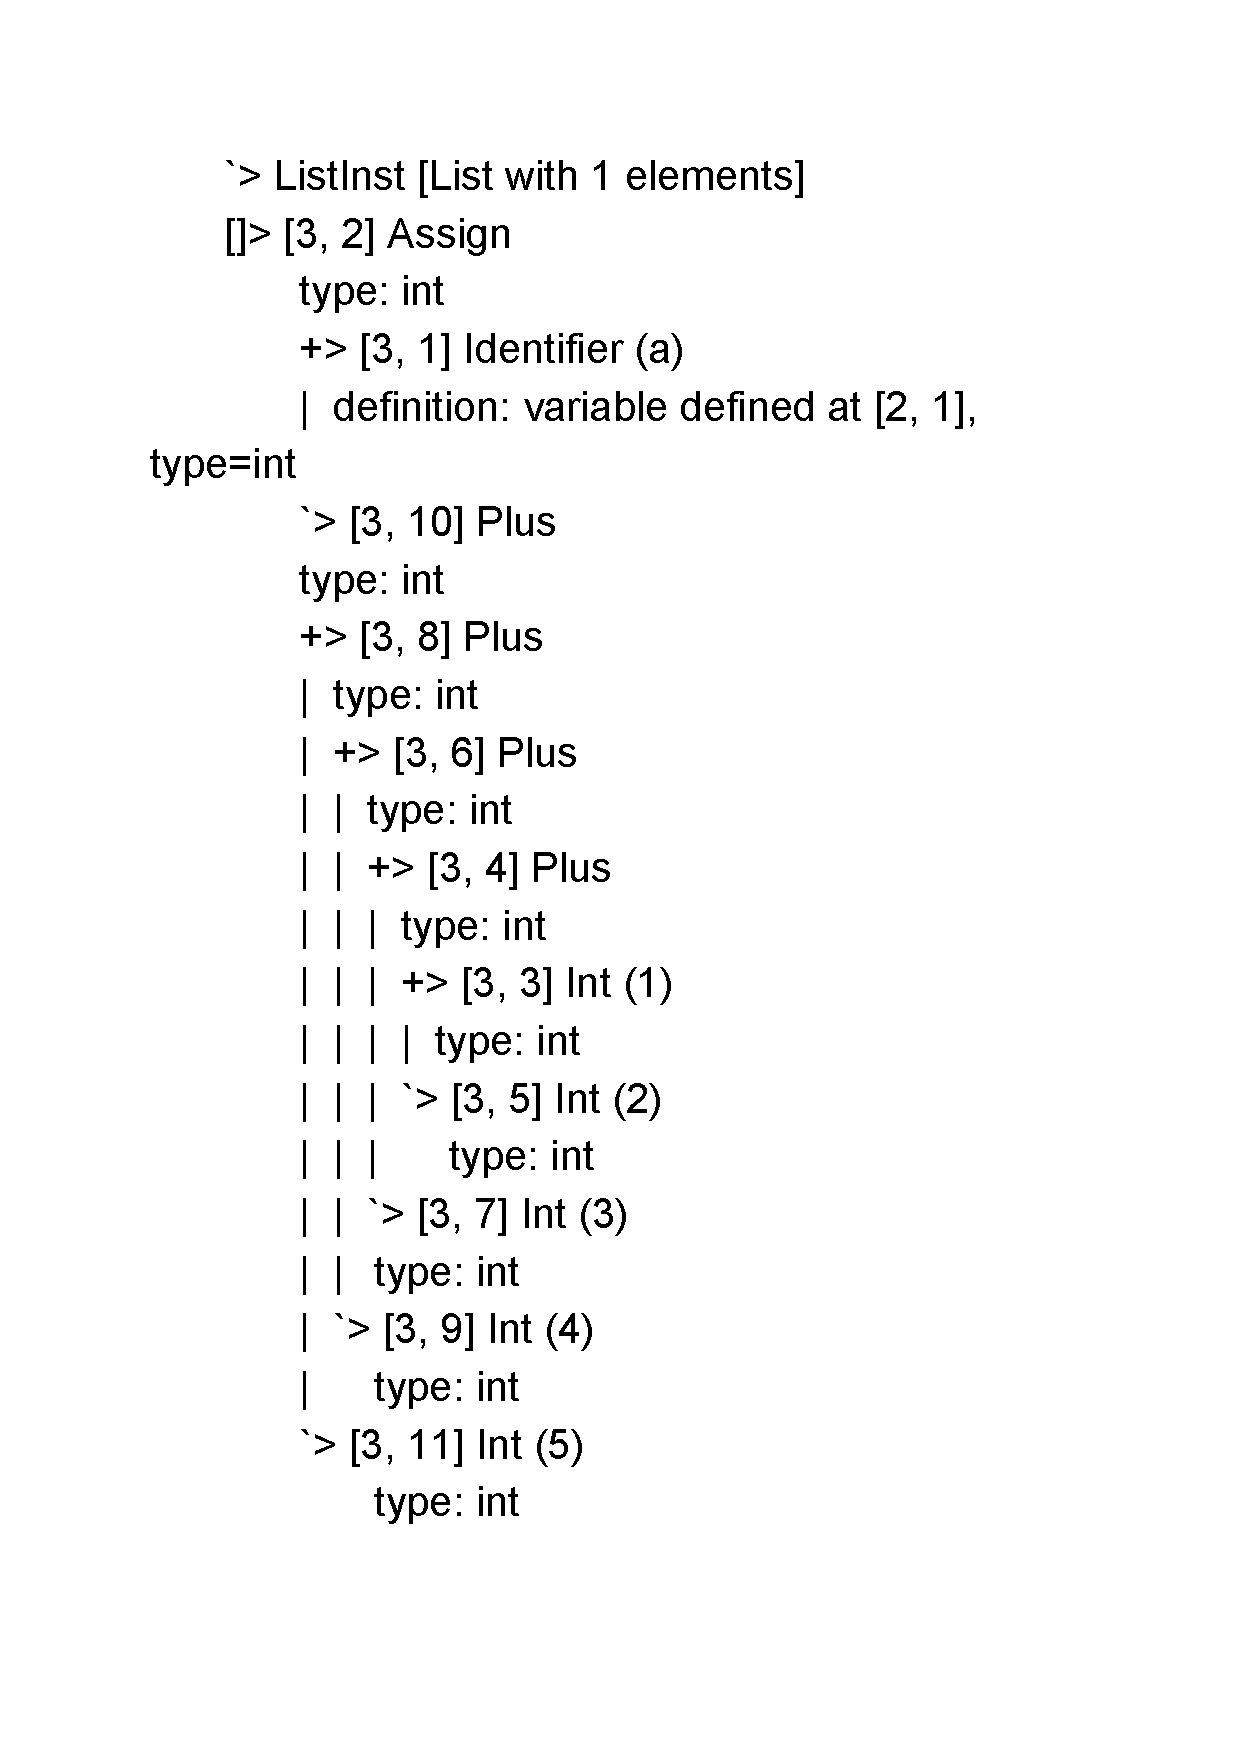
\includegraphics[scale=0.5]{Arbre_enrichi.pdf}\\
<<<<<<< HEAD
Une fois qu'on a stocké toutes les opérations et toutes les constantes dans ces $2$ listes il faut alors retirer la dernière opération du tableau et faire cette opération entre la valeur du résultat précédant (initialisé à 0) et la valeur du dernier élément constant du tableau qu'on aura aussi retiré (avec néanmoins un cas particulier à l'initialisation car il faut faire cette opération sur les deux derniers éléments du tableau).\\ \\
Une fois le résultat final calculé on set le fils de l'instruction que l'on est en train de traiter dans lequel on met un IntLiteral ou un FloatLiteral de la valeur que l'on vient de calculer. On peut ensuite passer à l'instruction suivante et tout recommencer jusqu'à la dernière instruction.\\ \\
Une fois les fonctionnalités implémentées, il suffit d'ajouter un attribut de type ConstantFolding appelé folding au decac compiler, rajouter une option de compilation $-o2$ pour mettre l'optimisation à true si on veut l'observer, et l'ajouter dans le main où sont situés la listinst, paramètres essentiels de notre optimisation.

\section{Méthode de validation}
Pour valider nos optimisations nous décompilons l'arbre que nous aurons optimisé au préalable. Nous effectuons donc la commande decac -p -o1 ou decac -p -o2 pour observer les optimisations au niveau du programme, ou les deux.
Les optimisations auront été fonctionnelles si l'on observe que le programme en sortie est différent que celui en entrée, on devrait ainsi voir les variables inutiles supprimées par exemple pour l'application du deadstore. Nous utilisons cette méthode sur des tests deca que nous avons écrit. Il y a tout de même quelques tests qui ne seront pas optimisé de manière à vérifier que l'optimisation n'efface pas malencontreusement des informations qui ne devraient pas être supprimées.
\section{Résultat}

\section{Améliorations possibles de l'extension et conseils pour maintenance}
Les optimisations proposées sont simples dans les démarches qu'elles exercent. Leur impact est peut-être mineur dans des programmes bien codés, mais peut-être plus utiles pour des codeurs débutants. Néanmoins on peut en tirer plusieurs enseignements.
En effet on peut désormais classifier les extensions selon plusieurs catégories: extension au niveau de la compilation (dont DeadStore et ConstantFolding), au niveau de l'exécution, au niveau de la mémoire etc...
On peut ainsi proposer une structure pyramidale des extension comme indiquée sur la photo ci-contre :\\
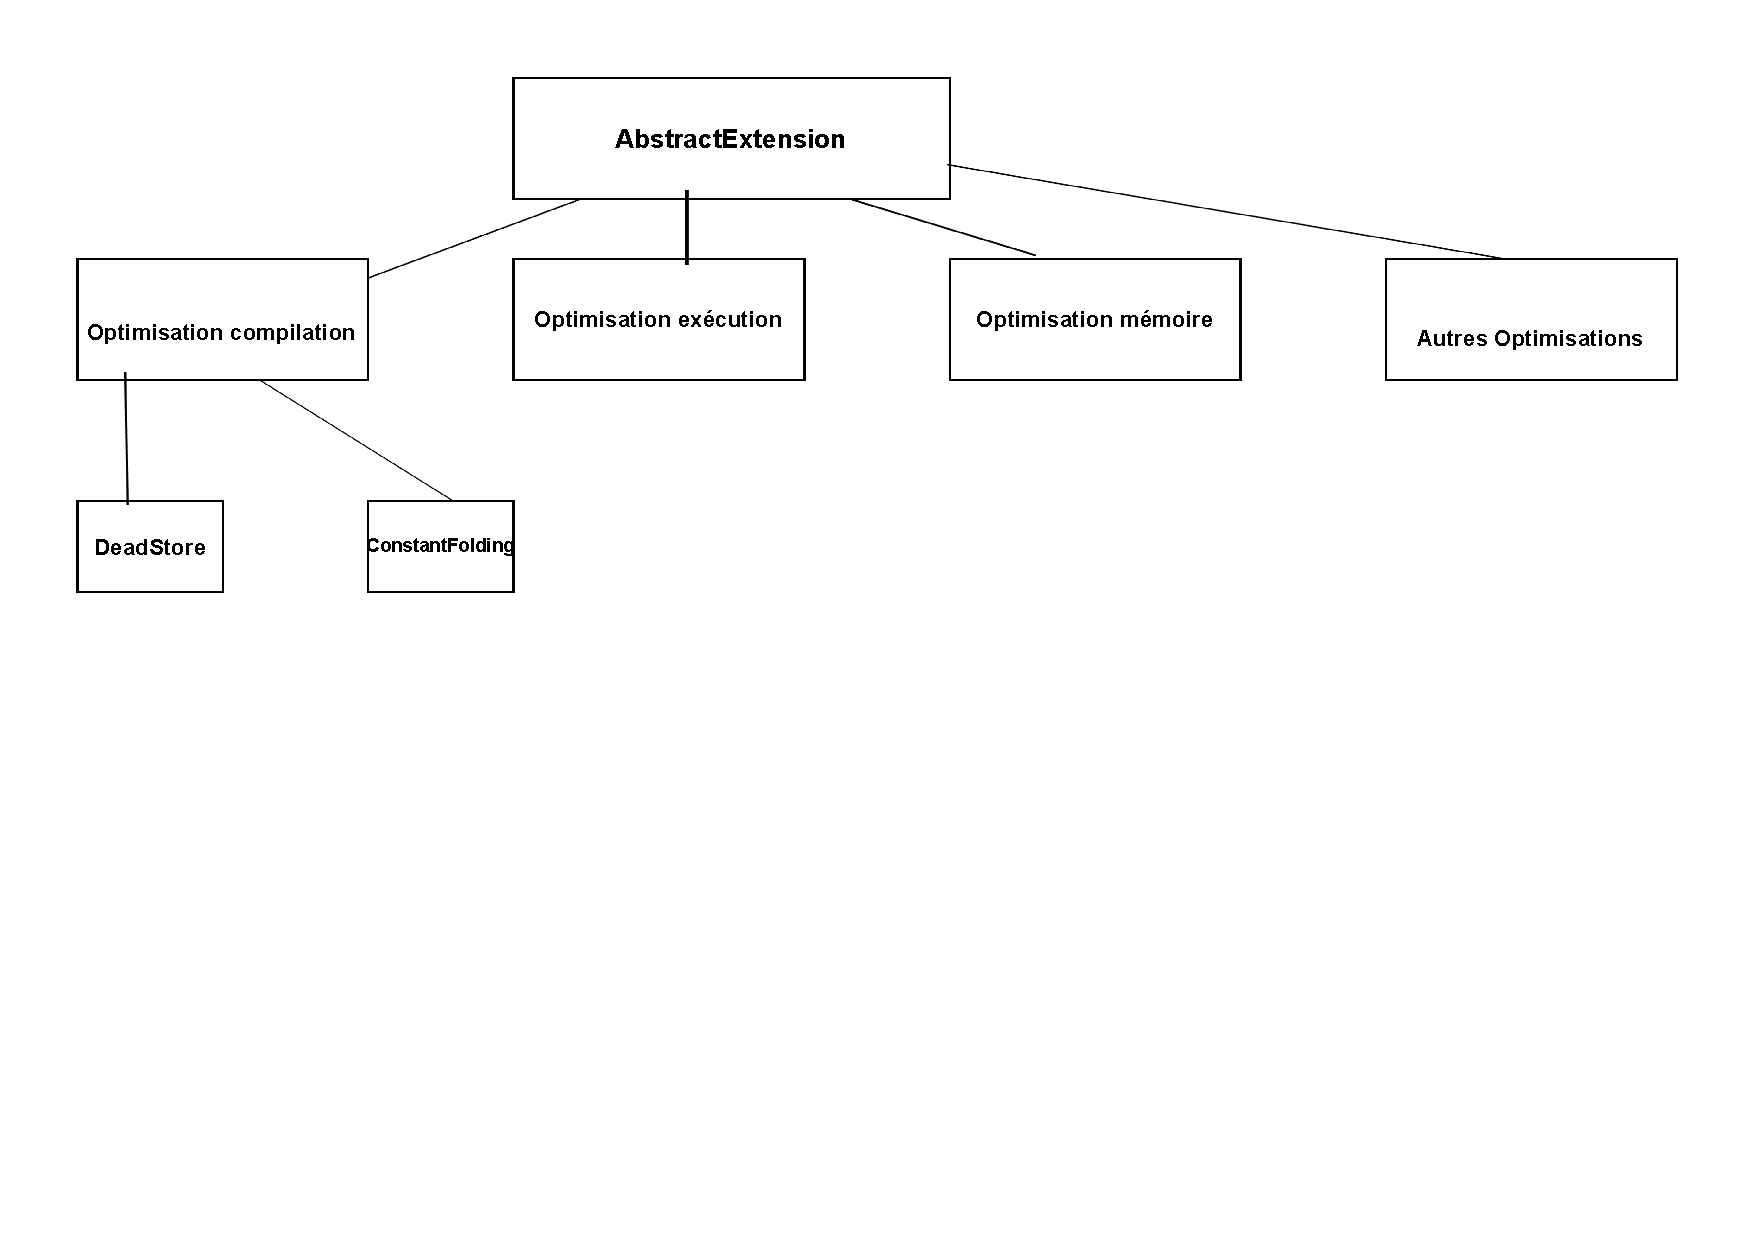
\includegraphics[scale=0.5]{UML.pdf}\\
Le futur programmeur qui voudra rajouter ses propres optimisations pourra ainsi créer ses propres classes, ses propres dépendances et ajouter les attributs qui lui sembleront nécessaires en essayant de respecter au mieux ce schéma proposé.
=======
Une fois qu'on a stocké toutes les opérations et toutes les constantes dans ces 2 listes il faut alors retirer la dernière opération du tableau et faire cette opération entre la valeur du résultat précédant (initialisé à 0) et la valeur du dernier élément constant du tableau qu'on aura aussi retiré (avec néanmoins un cas particulier à l'initialisation car il faut faire cette opération sur les deux derniers éléments du tableau).\\ \\
Une fois le résultat final calculé on set le fils de l'instruction que l'on est en train de traiter dans lequel on met un IntLiteral ou un FloatLiteral de la valeur que l'on vient de calculer. On peut ensuite passer à l'instruction suivante et tout recommencer jusqu'à la dernière instruction.\\ \\
Une fois les fonctionnalités implémentées, il suffit d'ajouter un attribut de type ConstantFolding appelé folding au decac compiler, rajouter une option de compilation $-o2$ pour mettre l'optimisation à true si on veut l'observer, et l'ajouter dans le main où sont situés les listdeclvar, paramètres essentiels de notre optimisation.

\section{Méthode de validation}
Pour valider nos optimisations nous décompilons l'arbre que nous aurons optimisé au préalable. Nous pourrons donc visualiser simplement si le dead store a correctement fonctionner, et de même pour le constant folding. Nous utilisons cette méthode sur des tests deca que nous avons écrit qui dont la plupart seront optimiséde manière à ce que la plupart soient optimisés. Il y a tout de même quelques tests qui ne seront pas optimisé de manière à vérifier que l'optimisation n'efface pas malencontreusement des informations qui ne devraient pas être supprimées.
\section{Résultat}

\section{Améliorations possibles de l'extension et conseils pour maintenance}
Les optimisations proposées sont simples dans les démarches qu'elles exercent. Leurs impacts est peut-être mineur dans des programmes bien codés, mais peut-être plus utiles pour des codeurs débutants. Néanmoins on peut en tirer plusieurs enseignements.
En effet on peut désormais classifier les extensions selon plusieurs catégories: extension au niveau de la compilation (dont DeadStore et ConstantFolding), au niveau de l'exécution, au niveau de la mémoire etc...
On peut ainsi proposer une structure pyramidale des extension comme indiquée sur la photo ci-contre :\\
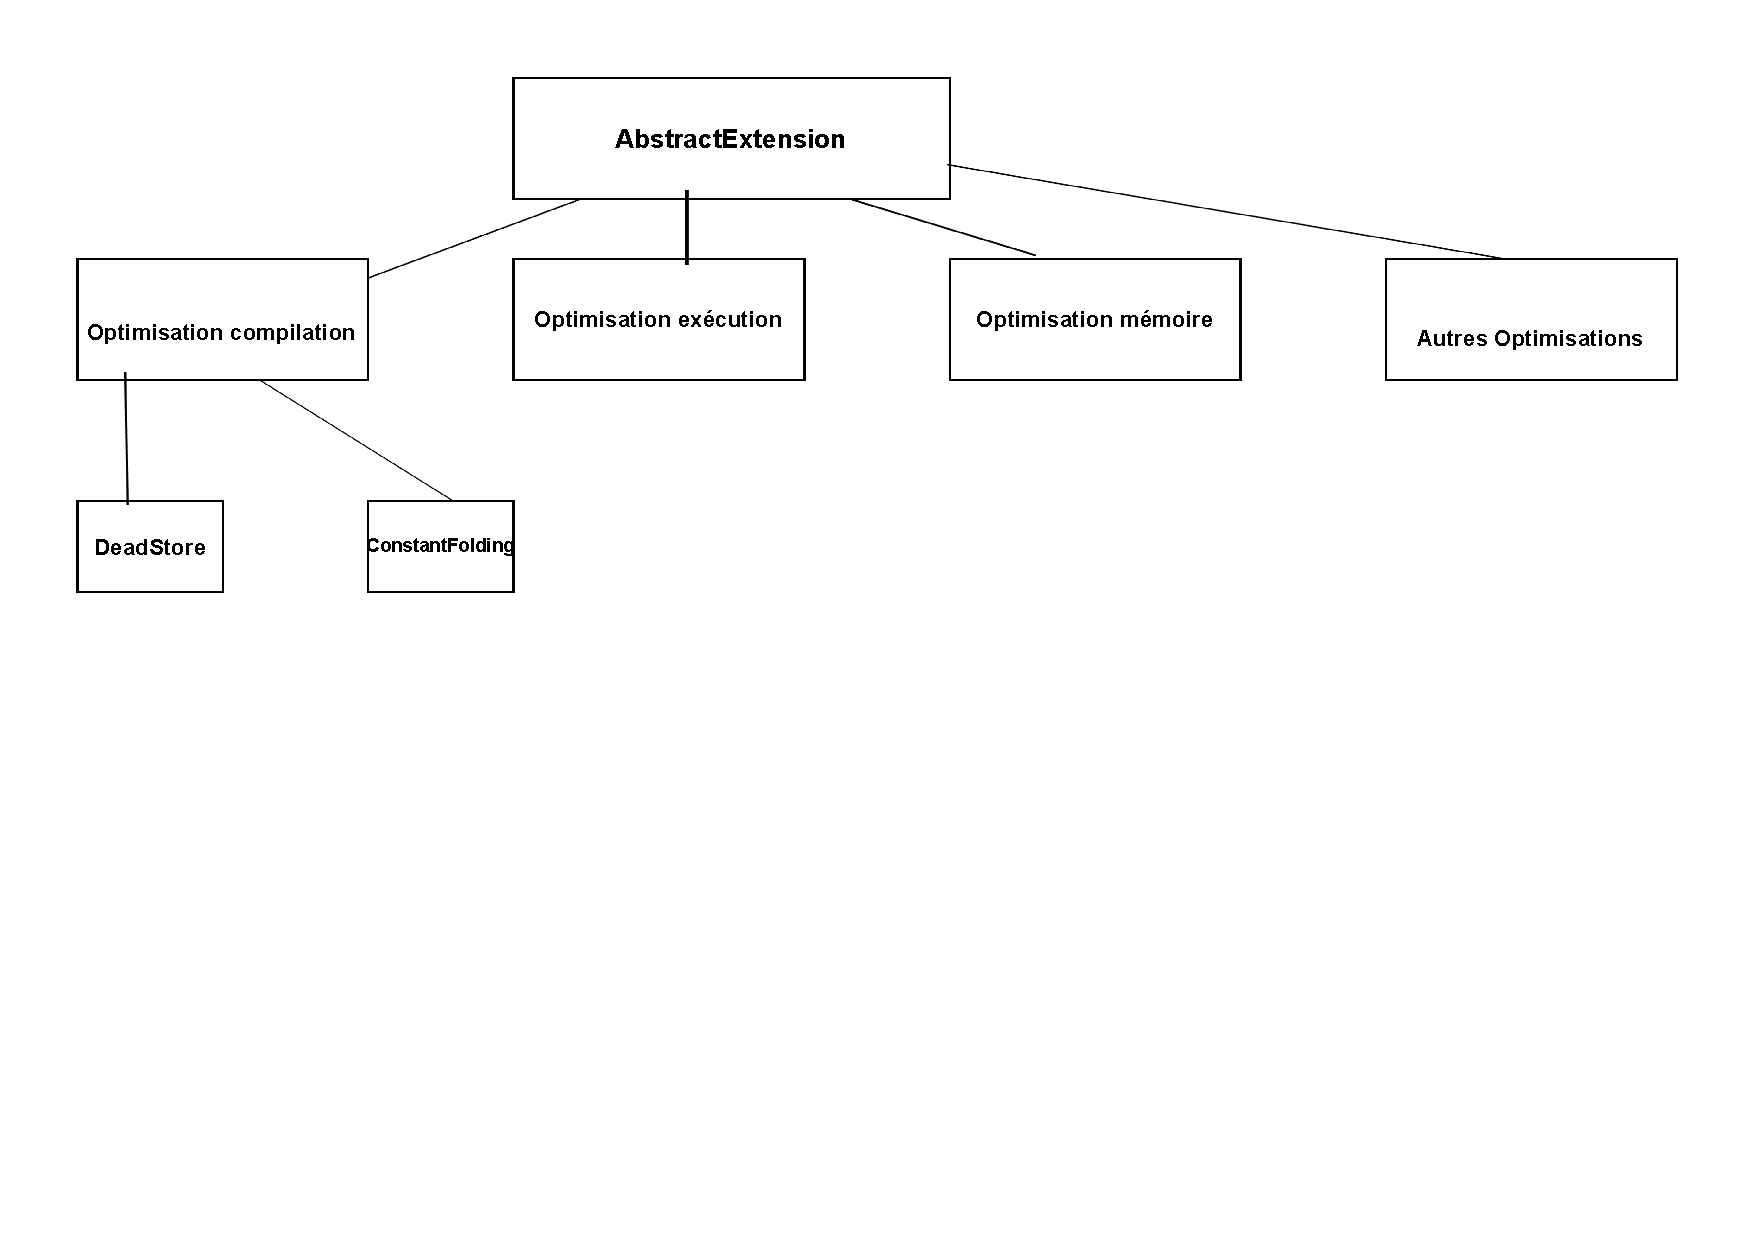
\includegraphics[scale=0.5]{UML.pdf}\\
Le futur programmeur qui voudra rajouter ses propres optimisations pourra ainsi créer ses propres classes, ses propres dépendances et ajouter les attributs qui lui sembleront nécessaires.
>>>>>>> aa1a17a2fb2cc9d7d8d1b313b725bf1e47fc4a09


\end{document}
